\section{Experiment details and ablation studies}
\label{appendix:experiment_details}
This section provides additional experimental details.

\subsection{Omitted Results}
Here, we present the comprehensive results on OpenWebText, on MAUVE score, Generative Perplexity (Gen PPL), and Entropy. The graph in Figure~\ref{fig:mauve-and-gen-ppl-plot} is derived from Table~\ref{tab:remdm-exp-owt}, PRISM-loop for $N>128$ and PRISM for $N=128$.

\begin{table*}[h]
\centering
\caption{Evaluation result for PRISM-loop/PRISM/baselines. The best MAUVE scores are \textbf{bolded}. \rebuttal{Baseline results marked with $^\dagger$ are taken from \cite{wang2025remasking}.}}
\label{tab:remdm-exp-owt}
\resizebox{\textwidth}{!}{%
\begin{tabular}{lccccccccc}
\toprule
Method & \multicolumn{3}{c}{MAUVE ($\uparrow$)} & \multicolumn{3}{c}{Gen PPL. ($\downarrow$)} & \multicolumn{3}{c}{Entropy ($\uparrow$)} \\
\midrule
Data & \multicolumn{3}{c}{1.00} & \multicolumn{3}{c}{14.8} & \multicolumn{3}{c}{5.44} \\
\midrule
& \textit{N=1024} & \textit{N=2048} & \textit{N=4096} & \textit{N=1024} & \textit{N=2048} & \textit{N=4096} & \textit{N=1024} & \textit{N=2048} & \textit{N=4096} \\
\midrule
MDLM$^\dagger$ & 0.042 & 0.037 & 0.035 & 51.3 & 51.3 & 50.9 & 5.46 & 5.46 & 5.45 \\
% MDLM+FB & 0.133 & 0.197 & 0.243 & 33.8 & 28.6 & 22.8 & 5.35 & 5.28 & 5.18 \\
% MDLM+DFM & 0.254 & 0.294 & 0.269 & 21.7 & 21.0 & 20.7 & 5.20 & 5.19 & 5.17 \\
ReMDM-conf & 0.051 & 0.060 & 0.065 & 48.0 &44.5 & 42.0 & 5.44 & 5.42 & 5.39 \\
ReMDM$^\dagger$ & 0.403 & 0.610 & \textbf{0.656} & 28.6 & 22.8 & 17.6 & 5.38 & 5.30 & 5.20 \\
\rowcolor{orange!25}
PRISM (ours) & 0.260 & 0.243 & 0.314 & 15.0 & 14.8 & 14.7 & 5.02 & 5.02 & 5.02 \\
\rowcolor{orange!25}
PRISM-loop (ours) & \textbf{0.527} & \textbf{0.632} & 0.548 & 15.3 & 14.3 & 13.6 & 5.10 & 5.08 & 5.08 \\
\midrule
& \textit{N=128} & \textit{N=256} & \textit{N=512} & \textit{N=128} & \textit{N=256} & \textit{N=512} & \textit{N=128} & \textit{N=256} & \textit{N=512} \\
\midrule
MDLM$^\dagger$ & 0.015 & 0.023 & 0.031 & 61.5 & 55.8 & 53.0 & 5.52 & 5.49 & 5.48 \\
% MDLM+FB & 0.064 & 0.084 & 0.100 & 42.8 & 39.6 & 37.1 & 5.44 & 5.41 & 5.38 \\
% MDLM+DFM & 0.041 & 0.144 & 0.211 & 37.9 & 26.5 & 23.3 & 5.31 & 5.26 & 5.23 \\
ReMDM-conf & 0.015 & 0.022 & 0.037 & 74.2 & 66.0 & 52.5 & 5.57 & 5.54 & 5.49 \\
ReMDM$^\dagger$ & 0.057 & 0.216 & 0.350 & 42.5 & 30.5 & 21.1 & 5.43 & 5.34 & 5.21 \\
\rowcolor{orange!25}
PRISM (ours) & \textbf{0.175} & 0.268 & 0.281 & 17.9 & 16.2 & 15.4 & 5.10 & 5.07 & 5.04 \\
\rowcolor{orange!25}
PRISM-loop (ours) & 0.118 & \textbf{0.294} & \textbf{0.423} & 21.5 & 18.0 & 16.4 & 5.18 & 5.15 & 5.12 \\
\midrule
& \textit{N=16} & \textit{N=32} & \textit{N=64} & \textit{N=16} & \textit{N=32} & \textit{N=64} & \textit{N=16} & \textit{N=32} & \textit{N=64} \\
\midrule
MDLM & 0.002 & 0.006 & 0.011 & 230.2 & 100.5 & 72.1 & 5.71 & 5.60 & 5.55 \\
% MDLM+FB & 0.064 & 0.084 & 0.100 & 42.8 & 39.6 & 37.1 & 5.44 & 5.41 & 5.38 \\
% MDLM+DFM & 0.041 & 0.144 & 0.211 & 37.9 & 26.5 & 23.3 & 5.31 & 5.26 & 5.23 \\
ReMDM-conf & 0.005 & 0.006 & 0.009 & 244.4 & 128.4 & 90.3 & 5.73 & 5.66 & 5.60 \\
ReMDM & 0.004 & 0.005 & 0.011 & 257.2 & 126.4 & 81.3 & 5.74 & 5.65 & 5.58 \\
\rowcolor{orange!25}
PRISM (ours) & \textbf{0.006} & \textbf{0.015} & \textbf{0.080} & 76.1 & 33.6 & 22.1 & 5.22 & 5.19 & 5.14\\
\rowcolor{orange!25}
PRISM-loop (ours) & 0.004 & 0.005 & 0.020 & 292.4 & 70.6 & 31.4 & 5.37 & 5.25 & 5.22 \\
\bottomrule
\end{tabular}
}
\vspace{-1.5ex}
\end{table*}

\subsection{Details on the remasking Strategy for OpenwebText}
\label{Appendix: owt inference ablations}
This section provides a detailed elaboration of the sampling strategies employed for the unconditional text generation in Section~\ref{sec:owt}. The main motivation for these interventions is to preserve sentence diversity, which is crucial for evaluated metrics.

\begin{itemize}[leftmargin=*,itemsep=0pt]
    \item \textbf{Staged Remasking}: We restrict the self-correction mechanism to be activated only after a specific step $\ell_{on}$.
    This restriction is motivated by the observation that low per-token quality scores in the initial sampling phase ($t>t_{\ell_{on}}$) are likely due to a lack of suffix context rather than token-level inaccuracies.
    Activating the correction mechanism only after a sufficient context prevents spurious modifications to an incomplete sequence.
    \item $\mathbf{\eta}$ \textbf{Inverse Scheduling}: Fixing $\eta$ was found to degrade the diversity as the $N$ increases.
    To mitigate this, an inverse scheduling rule was adopted, dynamically adjusting $\eta$ based on $N$.
\end{itemize}
To avoid complicated hyperparameter designs, we set these hyperparameters to be a function of $N$.
The remasking ratio and the remasking activation step are set to $\eta=\frac{2.56}{N}$ and $l_{on}=\lceil0.5N\rceil$, respectively. The $N$-step PRISM-loop algorithm comprises an initial $N/2$-step generation for the PRISM and then followed by an $N/2$-step loop with $M=20$.

\subsection{Ablation on Fine-tuning Hyperparameters-$(k,n_y)$}
\label{appendix: k_discussion}
\begin{figure}[h]
  \centering
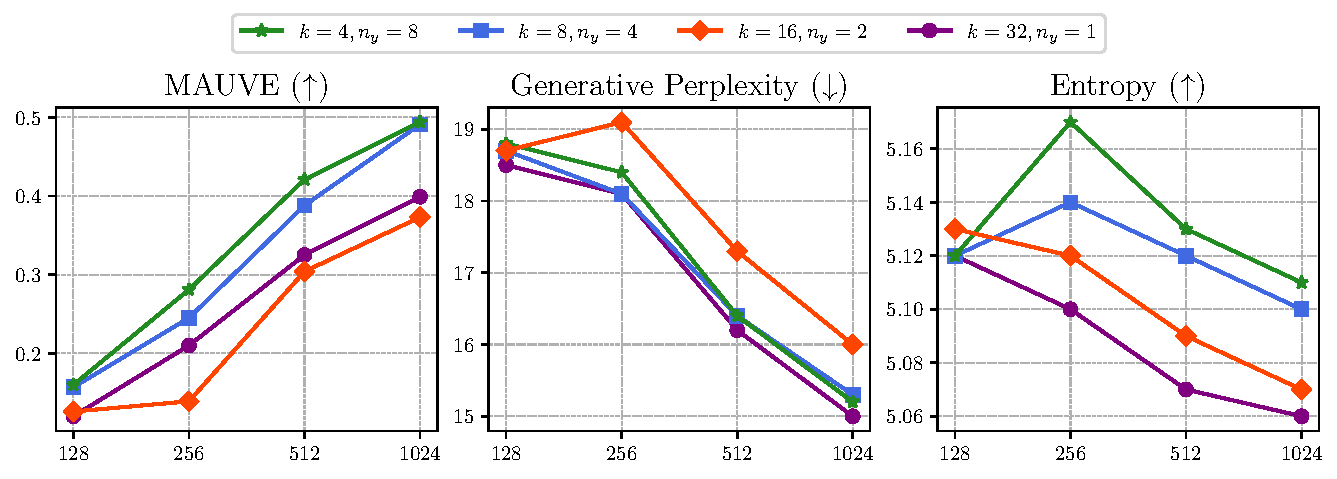
\includegraphics[width=\linewidth]{figs/ablation_kn_owt_plot.pdf}
  \caption{Ablation study on fine-tuning hyperparameters $k$ and $n_y$ while holding their product constant ($k \times n_y = 32$). Evaluations are conducted in ($128, 256, 512, 1024$) sampling steps.}
  \label{fig:ablation_kn_owt}
  \vspace{-1.0ex}
\end{figure}

In addition to $k$ (the number of tokens updated simultaneously to sample $\rvy$ from $\rvz$), we introduce a second hyperparameter, $n_y \in \mathbb{N}$, to improve data efficiency during the adapter's fine-tuning. As discussed in Section~\ref{sec:prism_empirical}, we can generate multiple distinct target sequences $\rvy$ from a single source sequence $\rvz$ by using different unmasking index sets $\mathcal{S}$. Therefore, $n_y$ denotes the number of unique unmasking sets applied per $\rvz$ in a single forward pass.

We conducted an ablation study to analyze how the interplay between $k$ and $n_y$ affects the generation performance.
We tested variants of $(k,n_y) \in \{(4,8), (8,4), (16,2), (32,1)\}$, thus remaining the total number of token updates per batch constant ($k \times n_y=32$) for a fair comparison.
All other configurations follow Table ~\ref{tab:configs}, except that we set nucleus $p=0.9$ to sample $\rvy$ from $\rvz$ (during the PRISM fine-tuning).

Our primary finding is that training the adapter with a smaller number of updating tokens (low $k$) results in a model that performs better at inference time, as measured by the MAUVE score.
This can be attributed to a train-test distribution mismatch induced by large $k$.
Specifically, updating many tokens simultaneously is likely to introduce joint dependency errors, increasing the chance of sampling a \emph{misleading} sequence $\rvy$.
This forces the adapter to train on a corrupted data distribution that is rarely encountered during inference time. Consequently, this mismatch leads to a poorly calibrated quality estimator, degrading the model's ability to perform effective self-correction.

\subsection{Ablation on Fine-tuning Hyperparameters-Nucleus sampling} \label{appendix:f_theta_discussion}
\begin{figure}[h]
  \centering
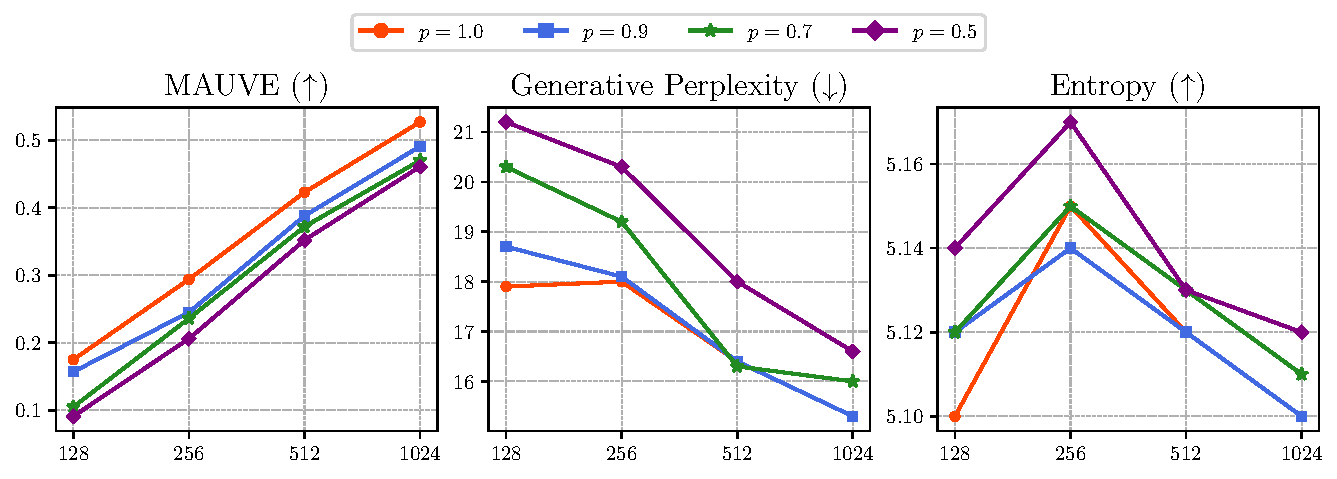
\includegraphics[width=\linewidth, height=0.2\textheight]{figs/ablation_p_owt_plot.pdf}
  \caption{Ablation study on nucleus sampling $p$ used to generate target sequences during adapter fine-tuning. Evaluations are conducted in ($128, 256, 512, 1024$) sampling steps. }
  \label{fig:ablation_p_owt}
  \vspace{-1.0ex}
\end{figure}

We further investigate how the sampling distribution used to generate target sequences $\rvy$ affects the adapter's fine-tuning process.
Specifically, we analyze the impact of nucleus sampling probability $p$ that we use to sample a token $\rvy^i$ from $f_\theta^i(\cdot\,|\,\rvz)$.
Our hypothesis is that a less restrictive sampling distribution (large $p$) is more beneficial for training the quality estimator than a shrunk one (small $p$).

Intuitively, a large $p$ induces a relatively diverse sample $\rvy$.
These sequences include not only high-probability tokens but also rare yet plausible alternatives. Training on these plausible-but-imperfect examples reduces exposure bias by forcing the model to calibrate its confidence across a wider range of outcomes, rather than only learning from its own single best predictions.
This process cultivates a more robust quality estimator capable of discerning subtle inaccuracies.
While this approach may introduce gradients with larger variance, it provides superior coverage of the complex distributions encountered during inference.
This ultimately leads to a more effective self-correction mechanism and improved text quality, as validated by the results in Fig.~\ref{fig:ablation_p_owt}.


\newpage
\subsection{Quantitative analysis of PRISM}
We provide the calibration analysis result of PRISM in Figure~\ref{fig:calibration_openweb}.
\begin{figure}[H]
    \centering
    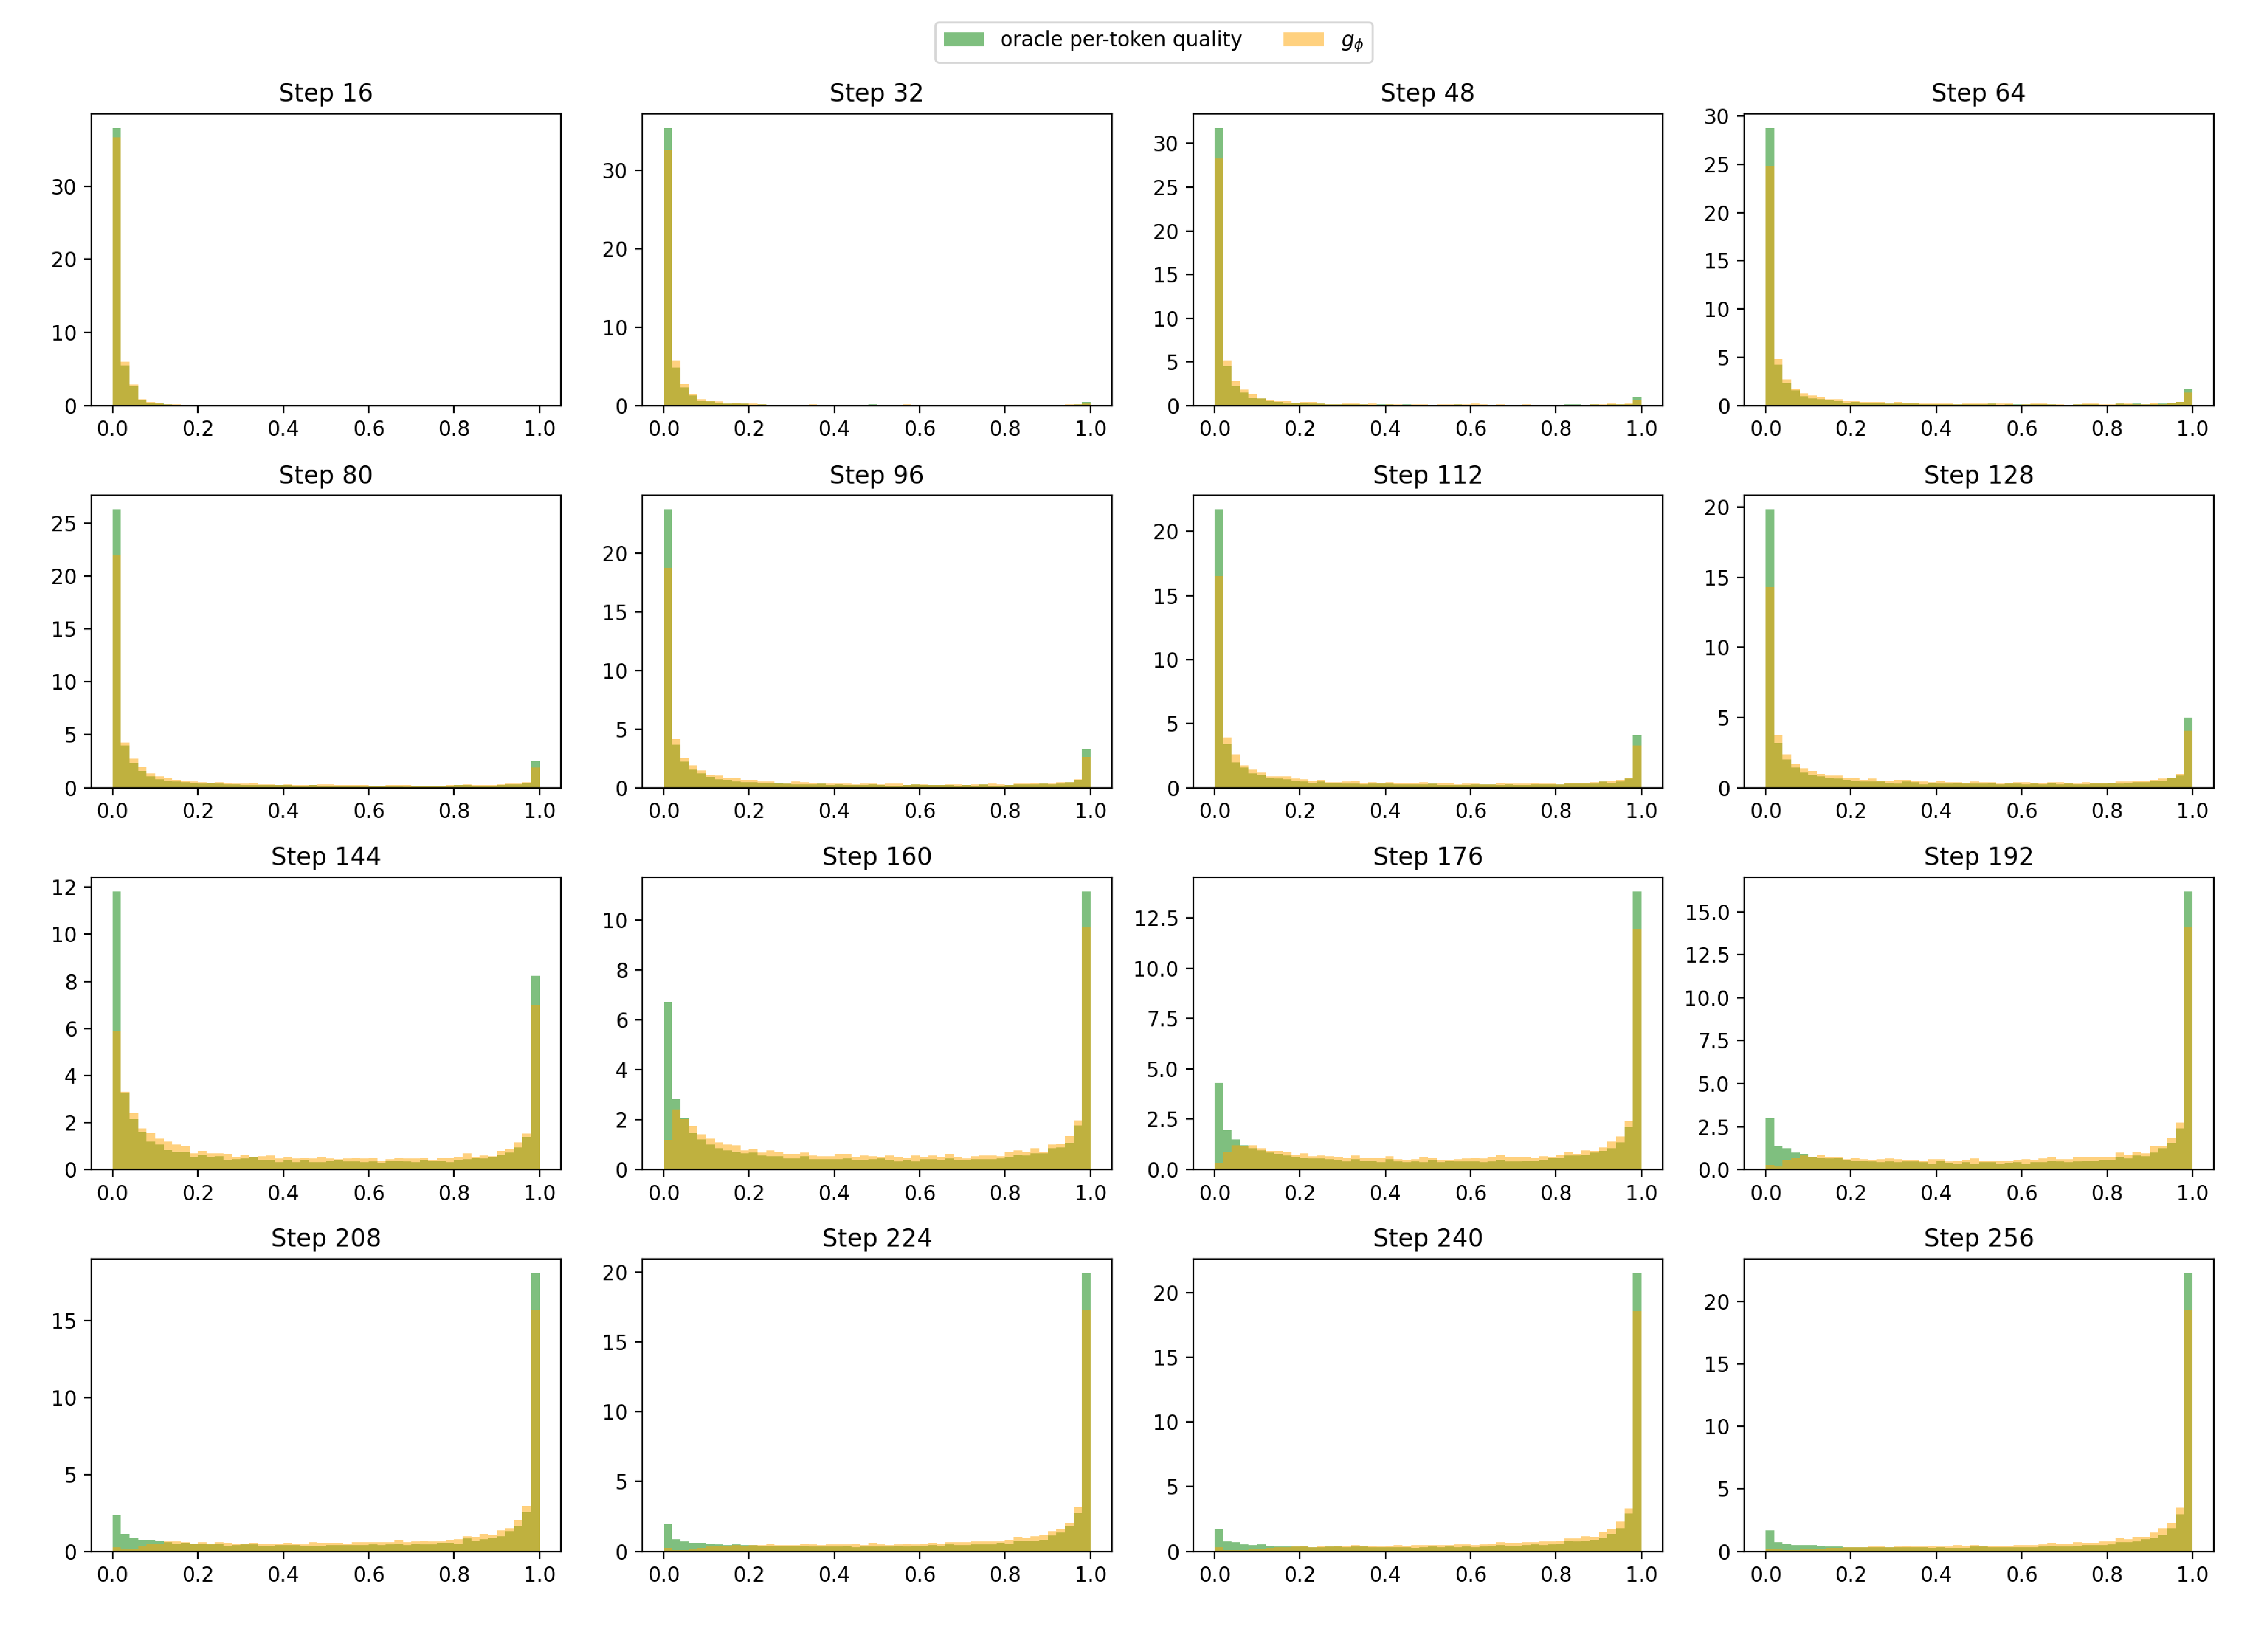
\includegraphics[width=0.75\textwidth]{figs/4x4_calibration_hist.pdf}
    \caption{
    \rebuttal{Calibration of PRISM per-token quality on OpenWebText during generation without remasking with $256$ steps.
    For each timestep, tokens are binned by predicted quality $g_\theta^i(\mathbf{x}_t)$, and for each bin we plot the empirical probability that token $i$ matches the ground truth, estimated via $f_\theta(\cdot \mid \mathbf{x}_t \oplus \mathbf{m}_i)$, against the bin mean.}
    }
    \label{fig:calibration_openweb}
\end{figure}

\subsection{Experiment Configurations}
\label{appendix: configs}
In Table~\ref{tab:configs}, we list the hyperparameter configurations for Sudoku, OWT, and LLaDA experiments.

\begin{table*}[h!]
\centering
\caption{Hyperparameter configurations for Sudoku, OWT, and LLaDA.}
\label{tab:configs}
\resizebox{0.8\textwidth}{!}{%
\begin{tabular}{lccc}
\toprule
\textbf{Hyperparameter} & \textbf{Sudoku} & \textbf{OWT} & \textbf{LLaDA} \\
\midrule
\multicolumn{4}{l}{\textbf{Base Model}} \\
\quad Architecture                & DiT & DiT & (non-causual) Transfomer\\
\quad Parameters                  & 28.6M & 169M & 8B\\
\quad Tokenizer                   & N/A & GPT-2 & LLaDA-8B-Instruct\\
\quad Sequence Length             & 81 & 1024 & 4096\\
\midrule
\multicolumn{4}{l}{\textbf{Fine-tuning}} \\
\quad Adapter Architecture        & linear & attention+linear & projection+linear \\
\quad Adapter Parameters          & 133K & 7.9M & 240M \\
\quad Optimizer                   & AdamW & AdamW & AdamW\\
\quad Learning Rate               & $3.0\times10^{-4}$ & $1.5\times10^{-4}$ & $1.0\times10^{-4}$ \\
\quad Weight Decay                & 0.0 & 0.0 & 0.1\\
\quad Gloabl Batch Size                  & 256 & 256 & 144\\
\quad $k$                         & 4 & 8 & 8 \\
\quad $n_y$                         & 1 & 4 & 1 \\
\quad Nucleus $p$                 & 1.0 & 1.0 & 0.0 \\
\quad $\lambda$             & 5.0 & 0.5 & 0.5 \\
\midrule
\multicolumn{4}{l}{\textbf{Sampling}} \\
\quad unmasking strategy          & random & random & semi-autoregressive \\
\quad $n_{\text{blocks}}$         & 1 & 1 & 32 \\
\quad Nucleus $p$                 & 1.0 & 0.9 & 0.0 \\
\quad Sampling Precision          & float64 & float64 & float32 \\
\quad $K$             & 4 & N/A & -- \\
\quad $l_{on}$       & 0 & $\lceil0.5N\rceil$ & -- \\
\quad $\eta$         & N/A & $\frac{2.56}{N}$ & N/A \\
\bottomrule
\end{tabular}
}
\vspace{-1.5ex}
\end{table*}

\subsection{Additional experimental details on LLaDA}
\label{appendix:llada}
Although Table~\ref{tab:configs} lists the basic configurations for our LLaDA experiments, we provide comprehensive details below.

\textbf{Attaching the adapter.}
As discussed in Section~\ref{sec:llada}, we freeze the LLaDA-8B-Instruct backbone and add (i) an auxiliary head to model per-token quality and (ii) a LoRA adapter on the qkv attention projections (rank $256$, dropout ratio $0.1$). This yields roughly $250$M trainable parameters in total.

\textbf{Dataset construction.}
For PRISM fine-tuning, we adopt the opc-sft-stage-2~\citep{Huang2024OpenCoderTO}, comprising $\approx 0.1$M challenging Python coding problems. Each example includes instructions and solutions. Thus, in the masking process, we do \emph{not} mask instruction tokens.

\textbf{Training configuration.}
We use AdamW~\citep{loshchilov2017decoupled} (learning rate \(1.0\times 10^{-4}\), weight decay \(0.01\), warmup ratio \(0.05\)) and use a cosine schedule with \(5\) cycles. Training for \(100\) epochs takes approximately \(30\) hours on \(12\) H100 GPUs.

\textbf{Inference details.}
For unmasking, we follow \citet{nie2025large} and employ semi-autoregressive inference: the sequence is partitioned into multiple blocks, and decoding proceeds from the leftmost block. We set the nucleus parameter to \(p=0.0\). These two choices are known to be important for competitive coding performance. 

For re-masking, across all baselines, we re-mask exactly $K_{\text{block}}$ tokens per block and schedule these re-masking operations at intermediate stages of block-wise inference (we observe degraded performance if re-masking is concentrated only at the beginning or end of a block). For a fair comparison, we report the best performance for PRISM and baselines (ReMDM, ReMDM-conf) over a sweep of $K_{\text{block}}$ at a fixed number of inference steps $N$: specifically,
\(K_{\text{block}}\in\{4,6\}\) for \(N=256\), (this is because the number of unmasking steps equals $8$ for $N=256$) and \(K_{\text{block}}\in\{8,10,12,14,16\}\) for \(N=512\) and \(N=1024\).
